% Generated by t15c05.py: 3-rank of the sandpile group of G(60,1/2), 1500 samples, against the limit law.
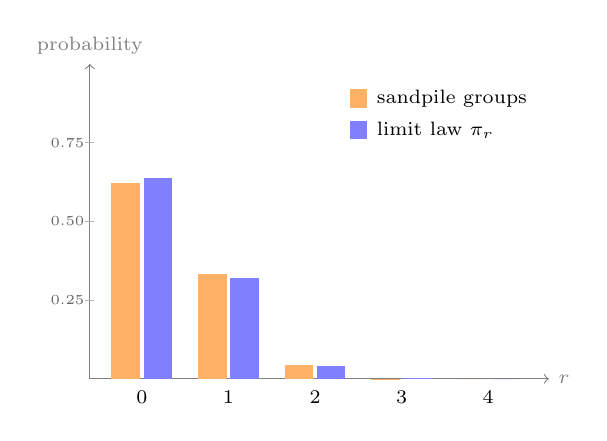
\begin{tikzpicture}[x=1.1cm,y=4cm]
\draw[->,black!50] (-0.6,0)--(4.7,0) node[right,font=\scriptsize]{$r$};
\draw[->,black!50] (-0.6,0)--(-0.6,1.0) node[above,font=\scriptsize]{probability};
\draw[black!30] (-0.65,0.25)--(-0.55,0.25) node[left,font=\tiny,black!60]{0.25};
\draw[black!30] (-0.65,0.50)--(-0.55,0.50) node[left,font=\tiny,black!60]{0.50};
\draw[black!30] (-0.65,0.75)--(-0.55,0.75) node[left,font=\tiny,black!60]{0.75};
\fill[orange!60] (-0.35,0) rectangle (-0.02,0.6233);
\fill[blue!50] (0.02,0) rectangle (0.35,0.6390);
\node[font=\scriptsize] at (0,-0.06) {0};
\fill[orange!60] (0.65,0) rectangle (0.98,0.3327);
\fill[blue!50] (1.02,0) rectangle (1.35,0.3195);
\node[font=\scriptsize] at (1,-0.06) {1};
\fill[orange!60] (1.65,0) rectangle (1.98,0.0433);
\fill[blue!50] (2.02,0) rectangle (2.35,0.0399);
\node[font=\scriptsize] at (2,-0.06) {2};
\fill[orange!60] (2.65,0) rectangle (2.98,0.0007);
\fill[blue!50] (3.02,0) rectangle (3.35,0.0015);
\node[font=\scriptsize] at (3,-0.06) {3};
\fill[orange!60] (3.65,0) rectangle (3.98,0.0000);
\fill[blue!50] (4.02,0) rectangle (4.35,0.0000);
\node[font=\scriptsize] at (4,-0.06) {4};
\fill[orange!60] (2.4,0.86) rectangle (2.6,0.92); \node[right,font=\scriptsize] at (2.6,0.89) {sandpile groups};
\fill[blue!50] (2.4,0.76) rectangle (2.6,0.82); \node[right,font=\scriptsize] at (2.6,0.79) {limit law $\pi_r$};
\end{tikzpicture}
